\chapter{Entwurfsmuster}

%% https://en.wikipedia.org/wiki/Software_design_pattern

\section{Singleton}

Das Singleton wurde für die beiden Klassen MariaDBConnector und JWTProvider eingesetzt.

\subsection{Einsatz begründen}

Das Singleton kam zum Einsatz da es gerantiert,
dass systemweit nur eine Instanz vorhanden ist und es nur eine einheitliche aktive Datenbank Verbindung geben soll.
Zudem benötigt das System auch nur eine globale Instanz des JWTProvider.
Weiterhin ermöglicht es einen einfachen Zugriff auf diese Instanz, ist einfach zu verstehen und anzuwenden.
Und eine Instanz wird auch nur angelegt wenn diese auch benötigt wird.
Durch das Singleton gibt es zwar keine Möglichkeiten für polymorpe Aufrufe mehr aber diese werden in diesem Fall auch nicht benötigt.


\subsection{UML}


\begin{figure}[htbp]
    \centering
    \fbox{
        
\includegraphics[width=4cm]{MariaDBConnector_before}
        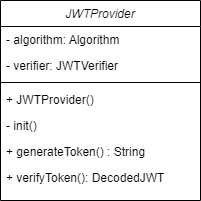
\includegraphics[width=4cm]{JWTProvider_before}
    }
    \caption{\label{1} UML vor Singleton}
\end{figure}

\begin{figure}[htbp]
    \centering
    \fbox{
        
\includegraphics[width=4cm]{MariaDBConnector_after}
        
\includegraphics[width=4cm]{JWTProvider_after}
    }
    \caption{\label{2} UML nach Singleton}
\end{figure}

